\chapter{Security Measures}\label{chapter:security_measures}
\todoin{Short intro text here}
\todoin{Description: Enumerate the security features your application uses and which attacks each feature defends against (specify which features you implemented and which you borrowed/use from other libraries)}

%Sample table
\securityMeasure{%
	%description
}{
	%implementation
}{
	%safe against
}


\subsection{HTTPS with HSTS}

\subsection{SSL secure ciphers}\label{sec:ssl_ciphers}
SSL ciphers are configured to the latest standards. As visible in \autoref{figure:ciphers1} and \autoref{figure:ciphers2}.
\begin{figure}[h!tbp]
	\centering
	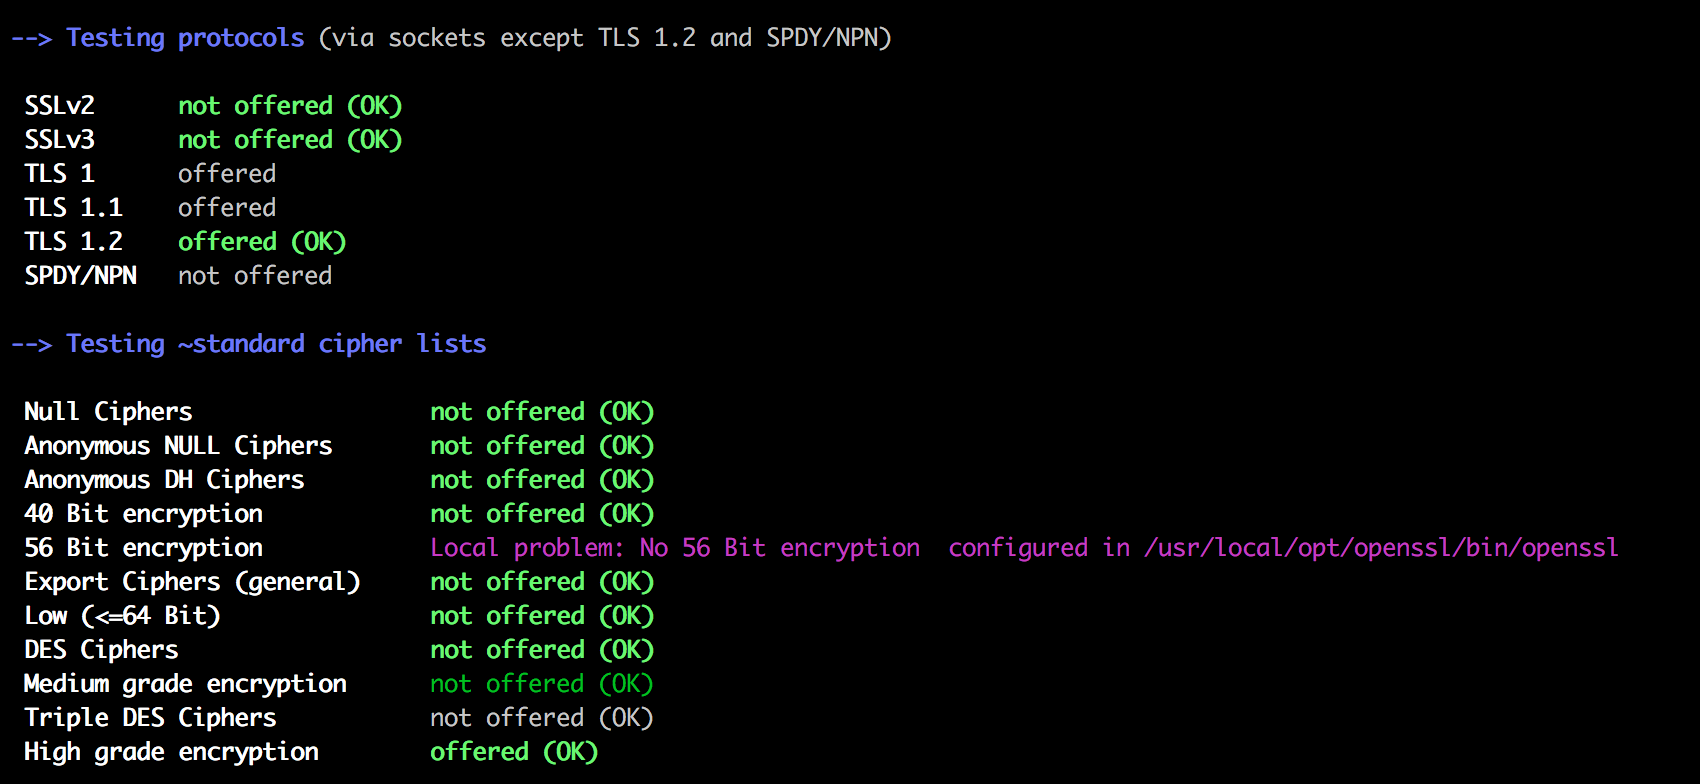
\includegraphics[width=\textwidth]{figures/ciphers1.png}
	\caption{Available SSL Ciphers}
	\label{figure:ciphers1}
\end{figure}
\begin{figure}[h!tbp]
	\centering
	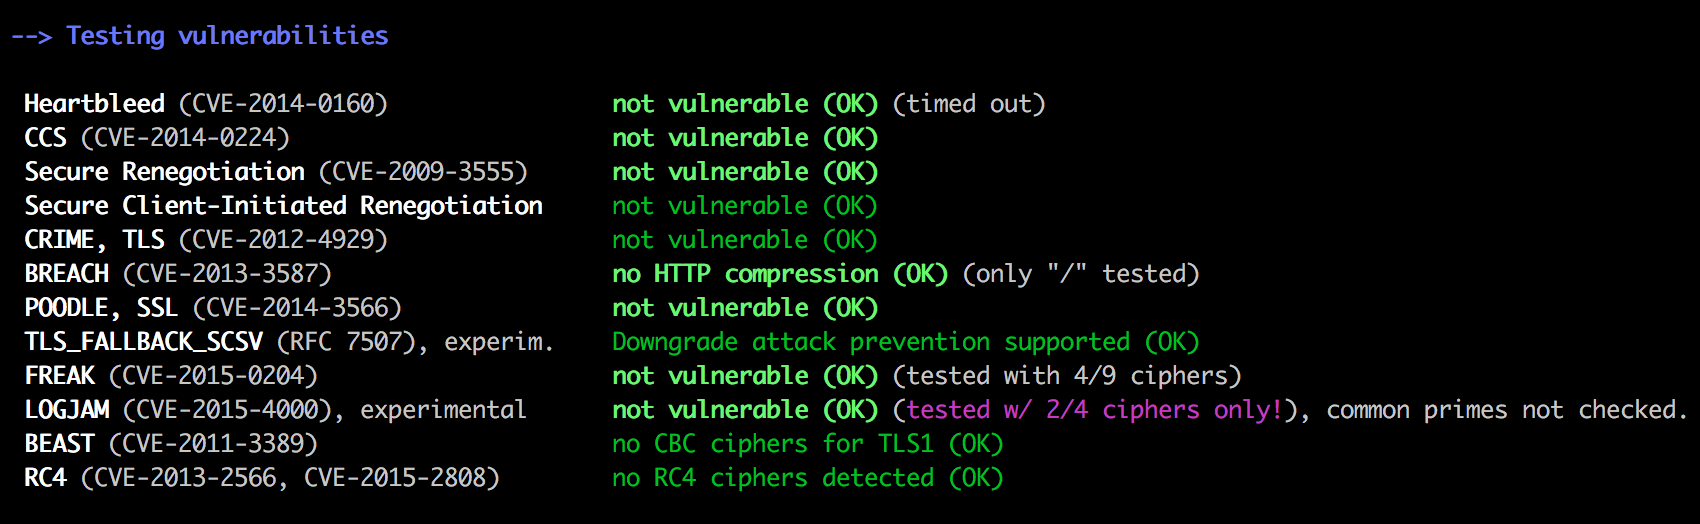
\includegraphics[width=\textwidth]{figures/ciphers2.png}
	\caption{No known SSL Vulnerabilities}
	\label{figure:ciphers2}
\end{figure}

\clearpage
\subsection{CSRF Tokens}
\securityMeasure{
	The application automatically creates anti-CSRF cryptographic nonces (tokens) on all pages with forms that could be exploited to perform operations using the profile of a user. These tokens are validated once the form is submitted by the user, ensuring that the application can't be forced to perform actions via cross-site requests.
}{
	This feature was implemented manually, by creating a 256-bit random token (obtained via the PHP builtin \texttt{openssl\_random\_pseudo\_bytes} function) and encoding it base64. This token is then saved as a session variable and sent to the user as a hidden field inside a form, as can be seen in the figure below. Once the form is submitted by the user, the the token contained inside the form is compared against the one already existing on the server.
}{
	This particular security feature protects against XSRF attacks, as described in OTG-SESS-005.
}
\begin{figure}[h!tbp]
	\centering
	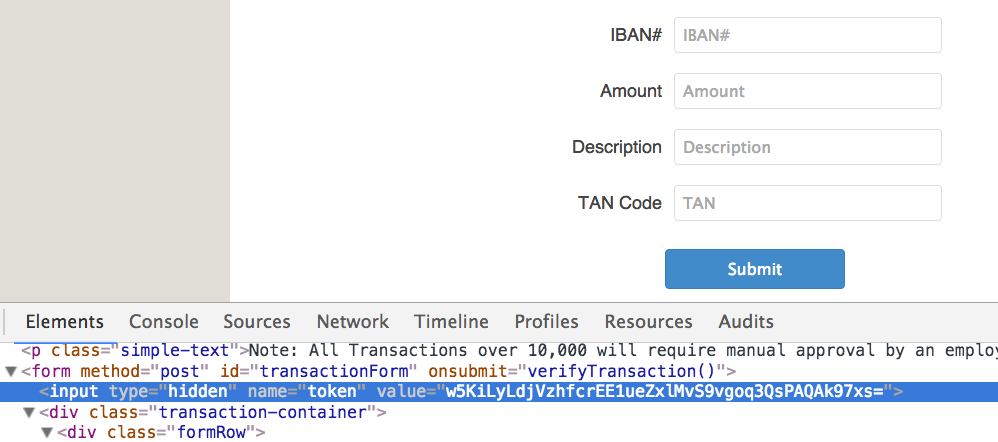
\includegraphics[width=\textwidth]{figures/csrf_token.png}
	\caption{CSRF token generated in the transaction page}
	\label{figure:csrf}
\end{figure}

\clearpage
\subsection{Password Strength}
%Sample table
\securityMeasure{%
	We enforce strong passwords by forcing the users to respect the following criteria:
	\begin{itemize}
		\item length between 8 and 20 characters;
		\item at least 1 numeric character (0-9);
		\item at least 1 upper/lower case letter (a-zA-Z);
		\item any special character inside the password is allowed.
	\end{itemize}
	Any password not matching these criteria is rejected by the server.
}{
	The password enforcing mechanism was manually implemented both on client side (see \texttt{project/js/registration.js}) and on server side (see \texttt{project/registration/registration\_request.php}). The user is compelled to follow the mentioned criteria when choosing a password during registration. This also holds true when resetting a password later on.
}{
	Strong password prevent attackers from guessing them, as described in OTG-AUTHN-007.
}

\clearpage
\subsection{Secure Passwords}
\securityMeasure{%
	User passwords are stored inside the database after a successful registration. Passwords are never stored in plaintext, but are hashed using a random salt, unique for every user, together with an additional static salt, known only to the backend server. 	
}{
	The algorithm used for hashing these values together is the SHA-512. A salt is generated for every user via the builtin PHP \texttt{openssl\_random\_pseudo\_bytes} function. The salt and the hashed password are both stored on the database (see \autoref{section:db}). No additional libraries were used to implement this feature.
}{
	Secure passwords protect the users in case the database is compromised in any way. An attacker is not able to determine which users are using the same passowrd and cannot retrieve the original password, starting from the hashed one.
}


\clearpage
\subsection{Password reset with two-factor authentication}

\clearpage
\subsection{Lockout mechanism after failed password entries}

\clearpage
\subsection{CAPTCHA}
\securityMeasure{%
	During the registration process users are required to enter a CAPTCHA code in order to prevent malicious attackers from automating registrations. This CAPTCHA is entirely random and requires the user to read an image an input the alphanumeric code manually.
}{
	For the creation of the CAPTCHA we resort to the \texttt{secureimage} library (see \ref{chapter:application_architecture} for further info).
}{
	This security feature protects the application from attackers who try to automate registrations (see OTG-IDENT-002), which could lead to a database saturation or even to a DOS.
}

\clearpage
\subsection{Balance calculated in database (Realtime concurrent transactions)}
... see \autoref{section:db} ...

\clearpage
\subsection{TANs in password protected PDFs}

\clearpage
\subsection{Time-based TANs generated via SCS}
